\section{Quick Introduction}

In this guide, we will detail the necessary steps for how to set up a \proglang{pbdR} environment.  What follows in the remaining sections is a very lengthy list of installation instructions; however, most users should find the process fairly straight-forward, and may not need (or want) all of the details we will provide unless something goes wrong.  In any case, the short version for setting up a pbdR environment is to:
\begin{enumerate}
  \item install \proglang{R} \incwin{(and Rtools for Windows)}\label{enum:r}; see \url{http://cran.r-project.org/}
  \item install an MPI library\label{enum:mpi}; \url{http://www.open-mpi.org/}, or \url{http://www.mpich.org/} for Windows
  \item install the pbdR packages; see \url{http://r-pbd.org/}
\end{enumerate}

Items \ref{enum:r} and \ref{enum:mpi} are interchangeable, and so if you already have \proglang{R} \incwin{(and additionally Rtools for Windows)} and/or an MPI library installed, then merely skip this/these step(s); there is no need to reinstall anything.

\subsection{Installing R}
This should be fairly painless.  \proglang{R} has binary packages for every operating system you have heard of (and some you haven't), and the install should go fine.  Of course, since \proglang{R} is open source, you are free to compile it yourself, should have have reason or need to do so.  You can find both the source as well as binaries at the \proglang{R} project's main site: \url{http://cran.r-project.org/}.  

Additionally, you may wish to customize your \proglang{R} build by compiling from source.  For example, you may wish to link \proglang{R} with a high performance linear algebra library, such as MKL.  See the \emph{R Installation and Administration Manual} at \url{http://cran.r-project.org/doc/manuals/R-admin.html} for full details.  


\subsection{Installing MPI}
\incmaclin{For Linux and Mac users, we recommend installing OpenMPI, which is available from \url{http://www.open-mpi.org/} in both binary and source formats.}  \incwin{Windows users should install MPICH2, available from  \url{http://www.mpich.org/} .} 


\subsection{Installing pbdR Packages}
All released pbdR packages are available from \url{http://cran.r-project.org/} which is the Comprehensive \proglang{R} Archive Network (CRAN).  This is similar to the CPAN for \proglang{perl} or CTAN for \LaTeX, although with many improvements and benefits over its competitors.

It is also possible to link pbdR with high performance linear algebra libraries, such as MKL.
\begin{figure}[h]
\centering
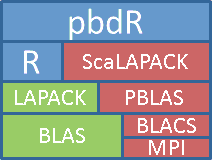
\includegraphics[scale=.7]{pics/libs.png}
\caption{pbdR Relationships to Libraries}\label{fig:pbd}
\end{figure}
Figure~\ref{fig:pbd} offers some insight into the package organization.  See the pbdSLAP vignette for more details.